% BEGIN LICENSE BLOCK
% Version: CMPL 1.1
%
% The contents of this file are subject to the Cisco-style Mozilla Public
% License Version 1.1 (the "License"); you may not use this file except
% in compliance with the License.  You may obtain a copy of the License
% at www.eclipse-clp.org/license.
% 
% Software distributed under the License is distributed on an "AS IS"
% basis, WITHOUT WARRANTY OF ANY KIND, either express or implied.  See
% the License for the specific language governing rights and limitations
% under the License. 
% 
% The Original Code is  The ECLiPSe Constraint Logic Programming System. 
% The Initial Developer of the Original Code is  Cisco Systems, Inc. 
% Portions created by the Initial Developer are
% Copyright (C) 2006 Cisco Systems, Inc.  All Rights Reserved.
% 
% Contributor(s): Kish Shen, IC-Parc
% 
% END LICENSE BLOCK
%
% $Id: embremoteproto.tex,v 1.3 2015/01/14 01:31:09 jschimpf Exp $
%
% Author:       Kish Shen, IC-Parc
%
\chapter{The Remote Interface Protocol}
\label{chapremoteproto}
%HEVEA\cutdef[1]{section}

\section{Introduction}

The {\eclipse} remote interface protocol is used to build a remote
interface between {\eclipse} and some programming language. A program
written in that programming language can interact and communicate with a
separate {\eclipse} process via the remote interface. The Tcl remote
interface (chapter~\ref{chapremote}) is an example of such an
interface. This chapter describes the protocol, so that remote interfaces
to other programming languages can be built.

The protocol is designed to allow the implementer to build an interface
that is compatible with the embedding interface of the same language. This
should allow the same code (in both {\eclipse} and the other language) to
be used in both interfaces. On the {\eclipse} side, the concept of {\it
peers\/} is used to unify the remote and embedding interfaces. 

Another feature of the remote interface is that on the {\eclipse} side,
the interface is independent of the programming language that is being
interfaced to. It should be possible to write {\eclipse} code with the
interface (e.g.\ for a GUI) and change the remote code without needing to
rewrite the code on the {\eclipse} side.

Briefly, a socket connection is established between the remote program and
an {\eclipse} process. The processes exchange messages in the EXDR (see
chapter~\ref{chapexdr}) format according to the protocol. This allows the
communication to be platform independent, and the {\eclipse} and remote
processes can be located on any two machines which can establish socket
connections. 

\section{Basics}
\label{remoteprotobasic}

The remote interface is established by {\bf attaching} the remote and
{\eclipse} processes. The attachment establishes two socket connections
between the two processes:

\begin{description}
\item[Control] This connection is used to control the remote
interface. Messages (in EXDR format) are sent in both directions according
to the remote protocol to co-ordinate the two processes.
\item[Rpc] This is used to send {\bf ec_rpc} goals from the remote process
to {\eclipse} and return the results. The goal is sent in EXDR format.
\end{description}

More than one remote attachment can be established in an {\eclipse}
process. Each attachment is independent, and is a remote peer,
identified by its control
connection. Each remote attachment has two sides: the {\eclipse} side, and
the remote side. 

At any one time, either the {\eclipse} or the remote side has {\it
control}. When a side has control, it is able to send messages to the other
side via the control connection. The side that does not have control
waits for messages to arrive on the control connection. On the {\eclipse}
side, execution is suspended while it does not have control. In general, once a
control message is sent, the control is passed to the other side, and the
side that sent the message waits for a reply message from the other side.

The {\bf ec_rpc} mechanism is designed to be the main way for the remote
side to interact with the {\eclipse} side. The remote side can send an
{\eclipse} goal, in EXDR format to be executed by the {\eclipse} side. This
can only be done while the remote side has control, and when the goal is
issued, a message is sent via the control connection to the {\eclipse}
side, and control is passed to the {\eclipse} side. Control is passed back
to the remote side when {\eclipse} completes the execution of the goal.

After the attachment, extra I/O connections can be established between the
two sides. This allows data to be transferred from one side to the other.
These connections (referred to as peer queues) can be of two types:

\begin{description}
\item[synchronous] These queues are synchronised by the control
connection. Control messages are exchanged between the two sides to ensure
that they are both are synchronised for the data transfer: one side
consumes the data that is sent from the other. This ensures that no
blocking occurs with the I/O operations across the sockets.

\item[asynchronous] These queues can perform I/O operations that are not
 co-ordinated by the control 
connection. Either side can write to or read from the queue 
without transferring control. In fact, if the remote language is
multi-threaded, it can perform asynchronous I/O while {\eclipse}
side has control. Note that asynchronous I/O
operations may block on the {\eclipse} side. 

\end{description}

\section{Attachment}
\label{remoteattach}
\subsection{Attachment Protocol}

\begin{figure}[hbt]
\begin{center}
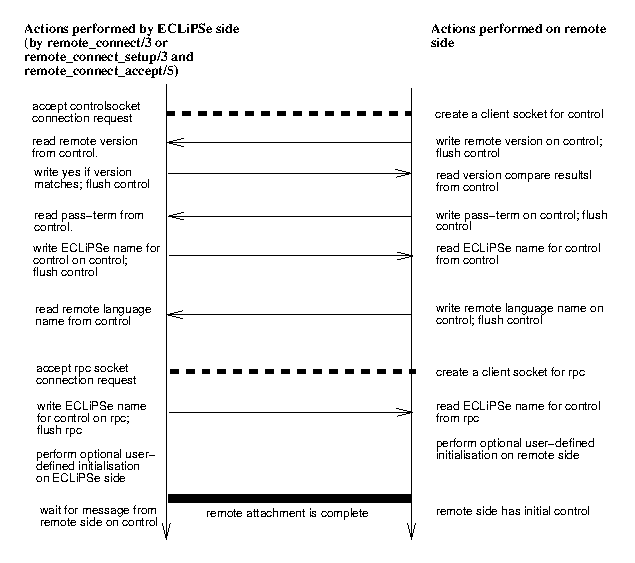
\includegraphics{remoteconnect.ps}
\end{center}
\caption{Summary of the attachment protocol}
\label{rattach}
\end{figure}


The attachment process is summarised in Figure~\ref{remoteattach}. It is
initiated from the {\eclipse} side, by either calling
\bipref{remote_connect/3}{../bips/kernel/externals/remote_connect-3.html} or the more flexible \bipref{remote_connect_setup/3}{../bips/kernel/externals/remote_connect_setup-3.html}
and \bipref{remote_connect_accept/6}{../bips/kernel/externals/remote_connect_accept-6.html} pair. In fact, {\bf remote_connect/3} is implemented using {\bf
remote_connect_setup/3} and {\bf remote_connect_accept/6} with default
values for some of the arguments. 

The attachment can be divided into several phases: 

\begin{enumerate}
\item Initialisation and handshaking: the control connection is
established, and handshaking between the two sides are carried out --
checking that the remote protocols on the two sides are compatible;
checking the pass-term.
\item Establishing the ERPC connections and exchange of information
(remote language, {\eclipse} name for the peer).
\item User-defined initialisations.
\end{enumerate}

The remote protocol version is stored in the flag {\tt
remote_protocol_version}, accessible via \bipref{get_flag/2}{../bips/kernel/env/get_flag-2.html}
as an integer version number.
This version number should only change when the protocol is
modified. Checking of the version ensures that the same (or at
least compatible) versions of the protocol are used, so that the two sides
behaves correctly. The version information is sent from the remote side
(which must have its own copy of the version information), and the
{\eclipse} side checks that this is compatible with the protocol version it
is using. In order to cope with remote connections which may not be using
the remote protocol, the {\eclipse} side waits only for a fixed period of
time for the remote side to send the version information before timing out.

Time-out on the {\eclipse} side can also occur for forming any of the
connections between the two sides, from the control connection to the peer
queue. This is specified by the user in {\tt remote_connect_accept/6}. If
time-out occurs during the attachment, then the attachment process is
abandoned, and the predicate fails (any connected sockets will be closed).

The detailed sequence of events for the attachment for the remote side
(with some description of the relevant {\eclipse} side actions) are:

\begin{enumerate}
\item {\eclipse} side: a socket server for the control connection is
created, using the address Host/Port which can be specified by the
user. It then waits to accept a socket stream for the control connection
from the remote side. The user can specify the amount of time to wait
before this operation times-out, which would then terminate the attachment.

\item Remote side: create a client socket stream for the control connection,
with an address compatible with Host/Port. The socket stream should
be in blocking mode, and perform no translation on the data sent.
\item Remote side: sends the remote protocol version information on the
control socket in EXDR format and flush it. This should be a {\tt
remote_protocol/1} term. 
\item {\eclipse} side: reads the EXDR version term from the control
socket, and compares with the version on the {\eclipse} side. If the two
protocols are compatible, it sends the EXDR string {\tt yes} back to
the remote side; otherwise it sends the {\eclipse} remote protocol version
to the remote side and disconnects from the remote side (raising
unimplemented functionality error). The {\eclipse} side waits at
most 100 seconds after the control connection is established for the remote side's version: after
this the {\eclipse} side disconnects the control connection and raises out
of range error. 
\item It is expected that the future versions of the protocol will remain
unchanged up to this point at least, to ensure the proper handshaking and
checking of versions.
\item Remote side: write the `pass-term' in EXDR format on the newly created control
connection and flush it. This provides a simple security check: {\eclipse}
side will check if the `pass-term' matches the `pass-term' it was given
when the remote connection was initiated -- for \bipref{remote_connect/3}{../bips/kernel/externals/remote_connect-3.html}, the
pass-term is the empty string, but the user can specify any pass-term if
\bipref{remote_connect_setup/3}{../bips/kernel/externals/remote_connect_setup-3.html} and \bipref{remote_connect_accept/6}{../bips/kernel/externals/remote_connect_accept-6.html} are
used. If the terms are not identical, then the {\eclipse} side will
discontinue the attachment process.

\item Remote side: read from the control connection the {\eclipse} name for the control
connection. This is sent in EXDR format, and is used to identify this
particular remote attachment -- the peer name for the peer. This name is needed when calling ec_rpc goals
that refer to the peer. 
\item Remote side: write the name of the programming language (e.g.\ tcl, java) of the
remote process on the control connection. This should be in EXDR string
format, and the connection flushed. 
\item {\eclipse} side: read the name of the programming language and store
it (it can be accessed later via \bipref{peer_get_property/3}{../bips/kernel/externals/peer_get_property-3.html}). The {\eclipse}
side now wait to accept the socket stream (using the same socket server as
the control connection) for the ec_rpc connection. This can also time-out.
\item Remote side: create a client socket stream for the ec_rpc connection, using the
same Port as for the control connection. This stream should be in
blocking mode, and perform no translation on the data sent. The server
socket on the {\eclipse} will be closed after accepting this client.
\item Remote side: read the control connection name again on the remote side, on the
newly established ec_rpc connection. This is also sent in EXDR format. This
is designed to verify that the ec_rpc connection is indeed connected to the
{\eclipse} side. 
\item Remote side: the remote side now has control. Any user-defined initialisations on the remote
side can now be performed, to make the remote side ready for the
interaction. The remote side has the control initially. Note that
user-defined initialisations on the {\eclipse} side is also performed after
sending the control name on the ec_rpc connection. After the
initialisation, {\eclipse} side will suspend and listen on the control
connection for the remote side to give control back to the {\eclipse} side.
\end{enumerate}

At the end of this, the remote side should be ready for normal interaction
with the {\eclipse} side.

The remote_connect/3 or remote_connect_accept/6 predicate waits for the control to be handed back by
the remote side before exiting. Thus when the predicate succeeds, the
remote side has been attached and properly initialised, with {\eclipse}
side having control.

The protocol does not specify how the remote side should be informed of the
Host/Port address for the initial socket connection. The Address can be
fixed before hand (with the Address argument instantiated, or
the information can be transmitted either manually or via files. In
addition, the remote process can be started from within {\eclipse} using
the \bipref{exec/3}{../bips/kernel/opsys/exec-3.html} command, with the host and port supplied as arguments.

In accepting client socket connections from the remote side, the {\eclipse}
side is informed of the host of the remote side. This should either be the
client's hostname, or 'localhost'. After accepting the control connection,
subsequent connections (for ec_rpc and any peer queues) are checked to
ensure that they are from the same client. If not, the attachment is
terminated by {\eclipse}. Using 'localhost' as the name on either side will
restrict the two sides to be on the same machine (and they must both use
localhost for Host in the address, rather than the actual hostname). 

\subsection{An example}

The following is a simple example of making a remote attachment on the
remote side. In this case, the remote side is also an {\eclipse} program.
A remote attachment by a program written in another programming language
will need to provide a similar function in that language:

\begin{verbatim}
% Example code for making a remote attachment on the remote side

:- local variable(ecsidehost).

% remote_attach/6 makes a remote attachment to a host ECLiPSe program.
% Args:
%    +Host: host name on ECLiPSe side
%    +Port: port on ECLiPSe side
%    +Pass: `pass-term' - used to verify the connection
%    +Init: goal to call to perform any application specific initialisation
%    -Control: the remote side (local) name of the control connection
%    -Ec_rpc:  the remote side name of the ec_rpc connection
%    -EcSideControl: the ECLiPSe side name for the control connection

remote_attach(Host, Port, Pass, Init, Control, Ec_rpc, EcSideControl) :-
     % control connection
     new_client_socket(Host, Port, Control),
     % send the protocol version information to the ECLiPSe side
     % we are the remote side, so must have our own version info.
     write_exdr(Control, remote_protocol(1)), flush(Control),
     % read response from ECLiPSe side to make sure it is compatible...
     read_exdr(Control, IsSameVersion),
     (IsSameVersion == "yes" ->
         true 
     ; 
         writeln("Incompatible versions of remote protocol. Failing...."),
         fail
     ),
     % send pass-term; if this does not match the pass-term on the ECLiPSe
     % side, it will terminate the attachment
     write_exdr(Control, Pass), flush(Control),
     % ECLiPSe side name for connection
     read_exdr(Control, EcSideControl),
     % send language name to ECLiPSe side
     write_exdr(Control, "eclipse"), flush(Control),
     % Ec_rpc connection
     new_client_socket(Host, Port, Ec_rpc),
     % read control name again on Ec_rpc to verify connection
     % in a more sophisticated implementation, this should time-out
     (read_exdr(Ec_rpc, EcSideControl) ->
        true 
     ; 
	% if not verified, terminate connection
        close(Control), close(Ec_rpc),
        fail
     ),
     % Remote side now has control, call Init to perform application
     % specific initialisations
     call(Init),
     % hand control over to ECLiPSe side...
     write_exdr(Control, resume), flush(Control).


new_client_socket(Host, Port, Socket) :-
     socket(internet, stream, Socket),
     connect(Socket, Host/Port).

%----------------------------------------------------
% the following code make use of remote_attach/6 to make an attachment,
% and then disconnect immediately when ECLiPSe side returns control

test(Host, Port) :-
     % make the remote attachment. For this simple example, there is no
     % application specific initialisations, and the default pass-term
     % of an empty string is used...
     remote_attach(Host, Port, "", true, Control, Ec_rpc, _),
     % control has been given to ECLiPSe side,
     % wait for ECLiPSe side to return control....
     read_exdr(Control, _),
     % immediately disconnect from ECLiPSe side
     write_exdr(Control, disconnect), flush(Control),
     % wait for ECLiPSe side to acknowledge disconnect...
     read_exdr(Control, disconnect_yield),
     % clean up
     close(Control), close(Ec_rpc).

\end{verbatim}

In addition to the attachment, the example contains a very simple example
of using the protocol by exchanging control messages with the {\eclipse}
side. After attachment, it disconnects the remote attachment as soon as
control is handed back to it. For more details on the messages, see next
section. 

To try out the example, start an {\eclipse} session and initiate a remote
attachment. This process is the {\eclipse} side:

\begin{verbatim}
(ECLiPSe side)
[eclipse 1]: remote_connect(Host/Port, Control, _).
Socket created at address chicken.icparc.ic.ac.uk/32436
\end{verbatim}

Now start another {\eclipse} session, compile the example program, and make
the attachment to the {\eclipse} side:

\begin{verbatim}
(Remote side)
[eclipse 4]: test('chicken.icparc.ic.ac.uk', 32436).
\end{verbatim}

On the {\eclipse} side, {\tt remote_connect/3} should now succeed:

\begin{verbatim}
(ECLiPSe side)
Host = 'chicken.icparc.ic.ac.uk'
Port = 32436
Control = peer3
yes.
[eclipse 2]: 
\end{verbatim}

The remote side is suspended, awaiting the {\eclipse} side to return
control. To return control to the remote side, the {\eclipse} side should
call \bipref{remote_yield/1}{../bips/kernel/externals/remote_yield-1.html} (see section~\ref{remotesupport} for a description
of {\tt remote_yield/1}):

\begin{verbatim}
(ECLiPSe side)
[eclipse 2]: remote_yield(peer3).
Abort
[eclipse 3]:
\end{verbatim}

In this simple example, when control is returned to remote side, it
immediately disconnects, thus the {\tt remote_yield/1} on the {\eclipse}
side is aborted (as disconnect was initiated from the remote side), as per
the disconnect protocol.

\begin{verbatim}
(Remote side)
[eclipse 4]: test('chicken.icparc.ic.ac.uk', 32436).

yes.
[eclipse 5]: 
\end{verbatim}

\section{Remote Peer Queues}

As discussed in section~\ref{remoteprotobasic}, peer queues can be formed
interactively during an attachment between the two sides. The protocol
provides for the creation and closing of these queues on both sides. 

The handling of data on these queues are performed by {\it data handlers},
routines which either provide data to the queue or consume data from the
queue. They are triggered by the appropriate control messages, so that a
data consumer handler would consume data arriving on a queue, and a data
provider handler would send data onto a queue (which would be consumed on
the other side). These data handlers can be user defined. 

The programmer for the remote side needs to provide the remote side of the
interface to the peer queue. 

\subsection{Synchronous peer queues}

The implementation of a synchronous peer queue on the {\eclipse} side is
shown in figure~\ref{syncpeer}. There is an in-memory buffer, which is
\begin{figure}[hbt]
\begin{center}
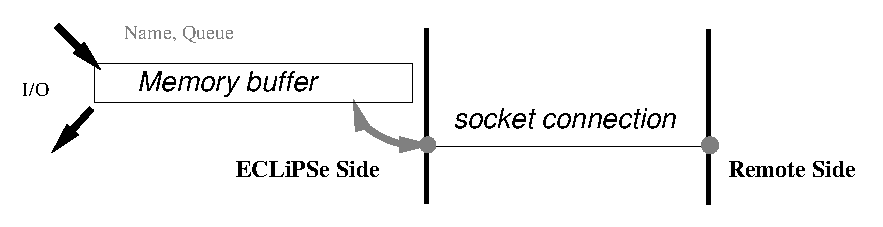
\includegraphics{syncpeer.ps}
\end{center}
\caption{{\eclipse} implementation of remote synchronous peer queue}
\label{syncpeer}
\end{figure}
implemented as a memory queue in {\eclipse} (i.e. {\tt queue("")} option
for \bipref{open/3}{../bips/kernel/iostream/open-3.html}). Associated with the memory queue is the actual socket
stream to the remote side.
The memory queue is the queue that the user sees on the {\eclipse}
side, with name {\it Name} and a unique integer id {\it Queue}, which is
the stream id for the memory queue. The id is used by both sides to identify
the queue, as it is unique (a symbolic name can always be reassigned), and
is used in the control messages. To conform to normal {\eclipse} streams,
these queues appear uni-directional to the user, i.e. data can be either
written to or read from the queue. The direction is {\it fromec} if the
direction of the data is from {\eclipse} to the remote side (i.e.\ 
{\eclipse} can output to the queue), and {\it toec}
if the direction is from the remote side to {\eclipse} (i.e.\ {\eclipse}
can read from the queue). The user perform normal I/O operations on the
memory queue, and the protocol ensures that the data is transferred
correctly to the remote side without blocking.

The socket stream is largely hidden from the user on the {\eclipse} side,
with data automatically transferred between it and the buffer. The buffer
is needed to ensure that when data is transferred between the two sides,
the I/O operation is synchronised (the data is being read on one end of the
socket while it is being written at the other), so no blocking will occur.
When a side needs to initiate an I/O operation with the other side (either
to write data to or read data from the other side via the socket stream), it must have control
(otherwise it would not be in a position to initiate an action). Before
performing the I/O operation, a control message is sent to the other side to
allow it to prepare to read the data before the I/O operation is actually
initiated. The memory queue thus serves to buffer the data before it is
transferred to the socket stream.

The socket stream must be connected to the remote side before it could be
used. Control messages are used also to synchronise the connection of
the socket. The protocol does not specify if a buffer is needed on the
remote side, this depends on the facilities available in the language used
for the remote side.

For a particular synchronous queue, a data handler can only be defined on
one side of the queue, but not both.
 
\subsection{Asynchronous peer queues}

I/O operations on these queues do not need to be controlled by the remote
protocol, but their creation and closing is controlled by the remote
protocol, so that the remote interface can keep track of these queues.
These are implemented as raw socket streams on the {\eclipse}
side, with I/O operations performed directly on the socket. The Name and
Queue id for the stream is thus those for the {\eclipse} socket stream. It
is the responsibility of the user to ensure that I/O operations do not
block on these queues. They are provided to allow asynchronous transfer of
data (e.g.\ from {\eclipse} side to the remote side without handing over
control), and also they allow more efficient transfer of data.  

\section{Control Messages}

These are the messages that are exchanged between the {\eclipse} and remote
sides when the remote side is attached. The messages are sent on the
control connection, and are in EXDR format. All arguments for the messages
are either atoms or integers. The messages are used to
co-ordinate and synchronise the two sides. A message should only be sent from a
particular side when that side has control, and control is handed over
to the other side when the message is sent. 

Most messages are used to initiate an {\it interaction\/} with the
other side. That is, used to cause some action to take place on the
other side: control is handed over, the action takes place on the other
side, and eventually control is handed back 
when the action is completed. Control can also be explicitly handed over
from one side to the other so that the other side can initiate
interactions. Some additional messages can only be sent as part of an
interaction, for exchanges of information between the two sides. Finally,
there are messages for terminating the remote attachment. Note that
interactions can be nested, that is, an interaction from one side can
contain an interaction initiated from the other side. 

The implementer for the remote interface should provide the methods for a
programmer to initiate the interactions from the remote side. These
routines would send the appropriate control messages to the {\eclipse}
side, and the messages should not be directly visible to the programmer. 

The usage of each message is summarised in the diagram(s) accompanying
them. These diagrams show:

\begin{itemize}
\item time proceeds downward. The {\eclipse} side is shown on the left,
the remote side on the right. Messages are shown as vertical arrows between
the two sides. The direction of the arrow indicates the direction the
message is sent.

\item the context in which the message can be sent, i.e.\ the message from
the other side that it is either expecting as a response, or that it is a
response to. The message sequence is shown, with the message highlighted.

\item any accompanying actions expected with the message. These actions are
either sending or receiving data on some other connections between the two
sides. These are shown as dashed arrows in the diagrams.

\item whether nested interactions can take place between messages of an interaction.
This is indicated by vertical ellipsis between the messages in
the diagram. In such cases, the nested interaction can be initiated, and this
interaction completed before the next message for the original interaction
is expected.
\end{itemize}

\subsection{Messages from {\eclipse} side to remote side}

 
\begin{description}
\item[yield] this yields control to the remote side.  The message is used either to
implicitly return control to the remote side at the end of an 
interaction initiated from the remote side, or it
is used to explicitly hand over control to the remote side. 


\begin{center}
% use toimage to generate images for hevea - _ needs to be \_
\begin{toimage}
\begin{picture}(200,70)
\thicklines
\put(70,52){\bf yield}
\put(20,50){\vector(1,0){150}}
\put(0,65){ECLiPSe}
\put(150,65){Remote}
\put(70,25){\shortstack{.\\.\\.\\.\\.\\.}}
\put(20,0){\line(0,1){65}}
\put(170,0){\line(0,1){65}}
\end{picture}
\begin{picture}(200,70)
\put(40,52){rpc {\footnotesize \it (goal via rpc)}}
\put(170,50){\vector(-1,0){150}}
\put(20,46){\dashbox{5}(150,0){}}
\put(20,46){\vector(-1,0){0}}
\put(20,10){\dashbox{5}(150,0){}}
\put(170,10){\vector(1,0){0}}
\thicklines
\put(40,16){{\bf yield} {\footnotesize \it (answer via rpc)}}
\put(20,14){\vector(1,0){150}}
\put(0,65){ECLiPSe}
\put(150,65){Remote}
\put(40,25){\shortstack{.\\.\\.\\.}}
\put(20,0){\line(0,1){65}}
\put(170,0){\line(0,1){65}}
\put(40,0){\shortstack{.\\.}}
\end{picture}
\begin{picture}(210,80)
\thicklines
\put(40,12){{\bf yield}}
\put(20,10){\vector(1,0){170}}
\thinlines
\put(20,46){\dashbox{5}(170,0){}}
\put(20,46){\vector(-1,0){0}}
\put(40,52){{\bf rem\_flushio(Q)} {\footnotesize \it (data via Q)}}
\put(190,50){\vector(-1,0){170}}
\put(0,65){ECLiPSe}
\put(170,65){Remote}
\put(40,25){\shortstack{.\\.\\.\\.}}
\put(20,0){\line(0,1){65}}
\put(190,0){\line(0,1){65}}
\put(40,0){\shortstack{.\\.}}
\end{picture}
\begin{picture}(210,80)
\thicklines
\put(40,12){{\bf yield}}
\put(20,10){\vector(1,0){170}}
\thinlines
\put(20,46){\dashbox{5}(170,0){}}
\put(20,46){\vector(-1,0){0}}
\put(30,52){{\bf rem\_flushio(Q,L)} {\footnotesize \it (L bytes via Q)}}
\put(190,50){\vector(-1,0){170}}
\put(0,65){ECLiPSe}
\put(170,65){Remote}
\put(40,25){\shortstack{.\\.\\.\\.}}
\put(20,0){\line(0,1){65}}
\put(190,0){\line(0,1){65}}
\put(40,0){\shortstack{.\\.}}
\end{picture}
\begin{picture}(210,60)
\put(40,32){queue\_close(Q)}
\put(170,30){\vector(-1,0){150}}
\thicklines
\put(40,12){\bf yield}
\put(20,10){\vector(1,0){150}}
\put(0,45){ECLiPSe}
\put(150,45){Remote}
\put(20,0){\line(0,1){45}}
\put(170,0){\line(0,1){45}}
\put(40,0){\shortstack{.\\.}}
\end{picture}
\begin{picture}(200,120)
\put(40,92){queue\_create(N,T,D,E)}
\put(170,90){\vector(-1,0){150}}
\put(40,77){socket\_client(P,N,T,D)}
\put(20,75){\vector(1,0){150}}
\put(40,62){socket\_connect(N,S)}
\put(170,60){\vector(-1,0){150}}
\put(40,47){socket\_accept(N,Q)}
\put(20,45){\vector(1,0){150}}
\put(40,32){resume}
\put(170,30){\vector(-1,0){150}}
\put(40,20){\shortstack{.\\.\\.}}
\thicklines
\put(40,12){{\bf yield}}
\put(20,10){\vector(1,0){150}}
\put(0,108){ECLiPSe}
\put(150,108){Remote}
\put(20,0){\line(0,1){105}}
\put(170,0){\line(0,1){105}}
\put(40,0){\shortstack{.\\.}}
\end{picture}
\end{toimage}
\imageflush
\end{center}

The interaction-initiating messages from the remote side will be described
in more detail in their own sections.

\item[ec_flushio(Queue, Length)] this message is sent when output on a remote
synchronous queue is flushed on the {\eclipse} side:

\begin{center}
\begin{toimage}
\begin{picture}(200,70)
\put(40,12){resume}
\put(190,10){\vector(-1,0){170}}
\put(20,46){\dashbox{5}(170,0){}}
\put(190,46){\vector(1,0){0}}
\thicklines
\put(40,52){{\bf ec\_flushio(Q,L)} {\footnotesize \it (L bytes via Q)}}
\put(20,50){\vector(1,0){170}}
\put(0,65){ECLiPSe}
\put(170,65){Remote}
\put(40,25){\shortstack{.\\.\\.\\.}}
\put(20,0){\line(0,1){65}}
\put(190,0){\line(0,1){65}}
\put(40,0){\shortstack{.\\.}}
\end{picture}
\end{toimage}
\imageflush
\end{center}

Queue is the
{\eclipse} stream number for the peer queue, and Length is the number of bytes
that is being sent on the queue. Control is yielded to the remote
side. The data on the queue Queue will be sent through the
queue after sending this message on the control connection, so on receiving
this message on the remote side, the remote side should read Length bytes from
Queue. After processing the data, the remote side should return
control to the {\eclipse} side via a {\bf resume} message.

\item[ec_waitio(Queue)] this message is sent when {\eclipse} requests input
from a remote synchronous queue, and the data is not available in the
queue's buffer. 

\begin{center}
\begin{toimage}
\begin{picture}(210,100)
\put(30,12){resume}
\put(190,10){\vector(-1,0){170}}
\put(30,32){yield}
\put(20,30){\vector(1,0){170}}
\put(20,56){\dashbox{5}(170,0){}}
\put(20,56){\vector(-1,0){0}}
\put(30,62){rem\_flushio(Q,L) {\footnotesize \it (L bytes via Q)}}
\put(190,60){\vector(-1,0){170}}
\thicklines
\put(30,82){{\bf ec\_waitio(Q)}}
\put(20,80){\vector(1,0){170}}
\put(0,95){ECLiPSe}
\put(170,95){Remote}
\put(20,0){\line(0,1){95}}
\put(190,0){\line(0,1){95}}
\put(30,70){\shortstack{.\\.}}
\put(30,40){\shortstack{.\\.\\.}}
\put(30,20){\shortstack{.\\.}}
\put(30,0){\shortstack{.\\.}}
\end{picture}
\begin{picture}(210,100)
\put(30,12){resume}
\put(190,10){\vector(-1,0){170}}
\put(30,32){yield}
\put(20,30){\vector(1,0){170}}
\put(20,56){\dashbox{5}(170,0){}}
\put(20,56){\vector(-1,0){0}}
\put(30,62){rem\_flushio(Q) {\footnotesize \it (data via Q)}}
\put(190,60){\vector(-1,0){170}}
\thicklines
\put(30,82){{\bf ec\_waitio(Q)}}
\put(20,80){\vector(1,0){170}}
\put(0,95){ECLiPSe}
\put(170,95){Remote}
\put(20,0){\line(0,1){95}}
\put(190,0){\line(0,1){95}}
\put(30,70){\shortstack{.\\.}}
\put(30,40){\shortstack{.\\.\\.}}
\put(30,20){\shortstack{.\\.}}
\put(30,0){\shortstack{.\\.}}
\end{picture}
\end{toimage}
\imageflush
\end{center}

This interaction is triggered when the {\eclipse} side attempts a read
operation on the empty buffer of a peer queue. The operation is suspended, 
and control is yielded to remote side so that it can provide
the required data. There should be a data-provider handler associated with
the queue on the remote side. This handler should obtain the data, and send
the data to the {\eclipse} side. The data will arrive from the remote side via a
{\bf rem_flushio} message, which initiates a remote flushio interaction, nested
within the {\eclipse} waitio interaction. The data arrives on the socket
associated with the remote peer queue Queue, and is automatically copied by
{\eclipse} into the peer queue buffer. Control is then yielded back to 
the remote side, completing the flushio interaction. The remote side then
hands control back to {\eclipse} side by the resume message. The suspended
read operation is resumed on the now non-empty buffer. 

The remote flushio interaction is described in more detail in its own
section. The main difference between a remote flushio initiated on the
remote side and one initiated by an {\eclipse} waitio described here is
that there must not be a data-consumer handler on the {\eclipse} side, as
the data is to be consumed by the suspended read operation instead.
This is ensured in the protocol by prohibiting handlers on both sides 
of a synchronous peer queue.

Note that the {\eclipse} side will also listen to the control connection
while waiting for the data to be sent from the remote side. If a {\bf
resume} is sent before the data arrives, this is likely caused by a
programming error in the data provider handler, which finished without
sending data to the {\eclipse} side. The {\eclipse} side will print a
warning message on the warning output stream, and immediately yield
back to the remote side. Other messages are handled as normal, recursively
while waiting for the data to arrive -- this is mainly intended to allow
for unexpected aborts from the remote side, although it could also be used to
perform ec_rpc calls before the remote side sends the data.

\item[socket_client(Port, Name, Type, Dir)] this requests the remote side
to form a client socket connection for the remote peer queue Name. The
queue is of type Type (sync or async), and direction Dir (fromec, toec for
synchronous queues, bidirect for asynchronous queues). The client socket is
to connect at port Port with the {\eclipse} side host name.  

\begin{center}
\begin{toimage}
\begin{picture}(200,100)
\put(40,52){socket\_connect(N,S)}
\put(170,50){\vector(-1,0){150}}
\put(40,37){socket\_accept(N,Q)}
\put(20,35){\vector(1,0){150}}
\put(40,12){resume}
\put(170,10){\vector(-1,0){150}}
\put(40,15){\shortstack{.\\.\\.}}
\put(40,0){\shortstack{.\\.\\.}}
\thicklines
\put(40,67){{\bf socket\_client(P,N,T,D)}}
\put(20,65){\vector(1,0){150}}
\put(0,88){ECLiPSe}
\put(150,88){Remote}
\put(20,0){\line(0,1){85}}
\put(170,0){\line(0,1){85}}
\end{picture}
\end{toimage}
\imageflush
\end{center}

The {\eclipse} side first creates a server socket for the peer queue Name.
The port address is Port. This, along with the details of the queue is
passed to the remote side via the {\bf socket_client} message. The remote side
should then connect a client socket with Port as the port, and the Host
used for the initial attachment (which is either localhost or the hostname
of the \verb'eclipse' side) for the host. 
It should also perform any additional
setups for the peer queue using the information sent with the message
(typically this involves setting up book-keeping information for the queue
on the remote side). When the remote side connection is established, it
returns control to {\eclipse} via a {\bf socket_connect} message:

\noindent
{\bf socket_connect(Name, Status)}

Name is the name of the queue, and should be the same as the Name sent by
the socket_client message. This is used to verify that the messages refer
to same interaction. The {\eclipse} side will raise an error and disconnect
from the remote side if the name does not match. Status is either 
success or fail, depending on if the remote side successfully created the
remote side of the queue or not.

If Status is success, then the {\eclipse} side will complete the connection
for the peer queue by accepting the socket connection. Since the remote end
of the socket exists, the accept operation should succeed very
quickly. If not, the operation will time-out, using the time-out interval
specified when the attachment was made. The server socket is closed
immediately after the accept operation. On successful connection,
{\eclipse} first checks that this client's host is indeed the same as the
one previously recorded for the remote side. If so, the
{\eclipse} will finish creating the {\eclipse} side of the queue. If not,
the connection is closed, and the operation is considered to have failed. 

If Status from the socket_connect message is fail,
then the {\eclipse} side will clean up the preparation for the peer queue. 

The {\eclipse} side then returns control to the remote side via a
{\bf socket_accept} message:

\noindent
{\bf socket_accept(Name,Queue)}

Name is again the name of the queue, and Queue the stream id. If the accept
was unsuccessful (or if Status for socket_connect was fail), then Queue
will be the atom fail, indicating that the peer queue connection was
unsuccessful. 

The remote side should then record the  id Queue for later use (it is
needed for the control messages connected with this peer queue). If instead
fail was received, then the remote side should clean up the attempted queue
connection. When the remote side has finished the final stage of the
connection, control is returned to the {\eclipse} side via a {\bf resume}
message, and the socket_client interaction completes.

Note that the {\bf socket_connect} and {\bf socket_accept} messages are
always exchanged during a socket_client interaction, even if the connection
failed on the remote side before {\bf socket_connect} is sent. They also
can only occur in this context. If these messages occur in any other
occasion, an error should be raised.

\item[queue_close(Queue)] this message is sent when the {\eclipse} side
closes the peer queue with id Queue. 

\begin{center}
\begin{toimage}
\begin{picture}(200,60)
\put(40,12){resume}
\put(170,10){\vector(-1,0){150}}
\thicklines
\put(40,32){{\bf queue\_close(Q)}}
\put(20,30){\vector(1,0){150}}
\put(0,45){ECLiPSe}
\put(150,45){Remote}
\put(20,0){\line(0,1){45}}
\put(170,0){\line(0,1){45}}
\put(40,0){\shortstack{.\\.}}
\end{picture}
\end{toimage}
\imageflush
\end{center}

The remote side should close the remote side of the peer queue Queue, and
remove all bookkeeping information associated with it. Control should then
be returned to {\eclipse} via a {\bf resume} message. The {\eclipse} side should
also close the queue and remove bookkeeping information on the {\eclipse} side.

\item[disconnect] this message is sent when {\eclipse} side initiates
disconnect. 

\begin{center}
\begin{toimage}
\begin{picture}(200,60)
\put(70,12){disconnect\_resume}
\put(170,10){\vector(-1,0){150}}
\thicklines
\put(70,32){\bf disconnect}
\put(20,30){\vector(1,0){150}}
\put(0,45){ECLiPSe}
\put(150,45){Remote}
\put(20,10){\line(0,1){35}}
\put(170,10){\line(0,1){35}}
\end{picture}
\end{toimage}
\imageflush
\end{center}

Control is yielded to the remote side, which should acknowledge
with the {\bf disconnect_resume} message. Once the {\eclipse} side receives this
message, the connection between the two sides is considered
terminated. The {\eclipse} side will then close all the connections (the
control and ec_rpc connections, and any asynchronous and synchronous
queues) to the remote side, and clean up the information associated with the
attachment. After sending the disconnect_resume message, the remote side
should also shutdown its end of the connection by closing all the
connections on its side. 

Note that the disconnection message can be used to terminate the attachment
from within an interaction. In such cases, the interaction(s) would not be
completed.

\item[disconnect_yield] this message is sent when {\eclipse} side receives
a {\bf disconnect} message from the remote side, i.e.\ the remote side
initiated disconnection. 

\begin{center}
\begin{toimage}
\begin{picture}(200,60)
\put(50,32){disconnect}
\put(170,30){\vector(-1,0){150}}
\thicklines
\put(50,12){\bf disconnect\_yield}
\put(20,10){\vector(1,0){150}}
\put(0,45){ECLiPSe}
\put(150,45){Remote}
\put(20,10){\line(0,1){35}}
\put(170,10){\line(0,1){35}}
\end{picture}
\end{toimage}
\imageflush
\end{center}

This message is sent as an acknowledgement to the
disconnect message. Once the disconnect_yield is sent, the connection is
considered terminated, and the {\eclipse} side will close all the
connections and clean up. After the clean up, abort is called. This is
done because the application on the {\eclipse} side (such as the remote
development tools) may be deep inside some interaction loop with the remote
side, and abort is the most general way of escaping from such a loop. It
can be caught (see \bipref{remote_yield/1}{../bips/kernel/externals/remote_yield-1.html} in section~\ref{remotesupport}) if
the user wants a more graceful termination. 


\end{description}

\subsection{Messages from remote side to {\eclipse} side}


\begin{description}

\item[resume] this message hands over control from remote side to
{\eclipse} side. This is used to either implicitly return control to the
{\eclipse} side at the end of an interaction initiated from the {\eclipse}
side, or to explicitly hand over control to the remote side.

\begin{center}
\begin{toimage}
\begin{picture}(200,70)
\thicklines
\put(70,52){\bf resume}
\put(170,50){\vector(-1,0){150}}
\put(0,65){ECLiPSe}
\put(150,65){Remote}
\put(70,25){\shortstack{.\\.\\.\\.\\.\\.}}
\put(20,0){\line(0,1){65}}
\put(170,0){\line(0,1){65}}
\end{picture}
\begin{picture}(200,70)
\put(40,52){ec\_flushio(Q,L) {\footnotesize \it (L bytes via Q)}}
\put(20,50){\vector(1,0){170}}
\put(20,46){\dashbox{5}(170,0){}}
\put(190,46){\vector(1,0){0}}
\thicklines
\put(40,12){\bf resume}
\put(190,10){\vector(-1,0){170}}
\put(0,65){ECLiPSe}
\put(170,65){Remote}
\put(40,25){\shortstack{.\\.\\.\\.}}
\put(20,0){\line(0,1){65}}
\put(190,0){\line(0,1){65}}
\put(40,0){\shortstack{.\\.}}
\end{picture}
\begin{picture}(210,110)
\put(30,82){ec\_waitio(Q)}
\put(20,80){\vector(1,0){170}}
\put(30,32){yield}
\put(20,30){\vector(1,0){170}}
\put(20,56){\dashbox{5}(170,0){}}
\put(20,56){\vector(-1,0){0}}
\put(30,62){rem\_flushio(Q,L) {\footnotesize \it (L bytes via Q)}}
\put(190,60){\vector(-1,0){170}}
\thicklines
\put(30,12){\bf resume}
\put(190,10){\vector(-1,0){170}}
\put(0,95){ECLiPSe}
\put(170,95){Remote}
\put(20,0){\line(0,1){95}}
\put(190,0){\line(0,1){95}}
\put(30,70){\shortstack{.\\.}}
\put(30,40){\shortstack{.\\.\\.}}
\put(30,20){\shortstack{.\\.}}
\put(30,0){\shortstack{.\\.}}
\end{picture}
\begin{picture}(210,110)
\put(190,10){\vector(-1,0){170}}
\put(30,82){ec\_waitio(Q)}
\put(30,32){yield}
\put(20,30){\vector(1,0){170}}
\put(20,56){\dashbox{5}(170,0){}}
\put(20,56){\vector(-1,0){0}}
\put(30,62){rem\_flushio(Q) {\footnotesize \it (data via Q)}}
\put(190,60){\vector(-1,0){170}}
\thicklines
\put(30,12){{\bf resume}}
\put(20,80){\vector(1,0){170}}
\put(0,95){ECLiPSe}
\put(170,95){Remote}
\put(20,0){\line(0,1){95}}
\put(190,0){\line(0,1){95}}
\put(30,70){\shortstack{.\\.}}
\put(30,40){\shortstack{.\\.\\.}}
\put(30,20){\shortstack{.\\.}}
\put(30,0){\shortstack{.\\.}}
\end{picture}
\begin{picture}(200,105)
\put(40,52){socket\_connect(N,S)}
\put(170,50){\vector(-1,0){150}}
\put(40,37){socket\_accept(N,Q)}
\put(20,35){\vector(1,0){150}}
\put(40,67){socket\_client(P,N,T,D)}
\put(20,65){\vector(1,0){150}}
\put(40,15){\shortstack{.\\.\\.}}
\put(40,0){\shortstack{.\\.\\.}}
\thicklines
\put(40,12){\bf resume}
\put(170,10){\vector(-1,0){150}}
\put(0,88){ECLiPSe}
\put(150,88){Remote}
\put(20,0){\line(0,1){85}}
\put(170,0){\line(0,1){85}}
\end{picture}
\begin{picture}(200,60)
\put(40,32){queue\_close(Q)}
\put(20,30){\vector(1,0){150}}
\thicklines
\put(40,12){\bf resume}
\put(170,10){\vector(-1,0){150}}
\put(0,45){ECLiPSe}
\put(150,45){Remote}
\put(20,0){\line(0,1){45}}
\put(170,0){\line(0,1){45}}
\put(40,0){\shortstack{.\\.}}
\end{picture}
\end{toimage}
\imageflush
\end{center}

\item[rpc] this message is sent before the remote side sends an ec_rpc goal
on the rpc connection. 

\begin{center}
\begin{toimage}
\begin{picture}(200,70)
\put(40,16){yield {\footnotesize \it (answer via rpc)}}
\put(20,14){\vector(1,0){150}}
\put(20,46){\dashbox{5}(150,0){}}
\put(20,46){\vector(-1,0){0}}
\put(20,10){\dashbox{5}(150,0){}}
\put(170,10){\vector(1,0){0}}
\thicklines
\put(40,52){{\bf rpc} {\footnotesize \it (goal via rpc)}}
\put(170,50){\vector(-1,0){150}}
\put(0,65){ECLiPSe}
\put(150,65){Remote}
\put(40,25){\shortstack{.\\.\\.\\.}}
\put(20,0){\line(0,1){65}}
\put(170,0){\line(0,1){65}}
\put(40,0){\shortstack{.\\.}}
\end{picture}
\end{toimage}
\imageflush
\end{center}

After sending the {\bf rpc} message, the remote side
should then send the ec_rpc goal (in EXDR format) on the rpc
connection. When the execution of the ec_rpc goal is finished, the
{\eclipse} side will yield control back to the remote side with a {\bf
yield} message, followed by the result of the ec_rpc execution on the rpc
connection (in EXDR format) -- the goal with its bindings if the execution
succeeded; `fail' if the goal failed; `throw' if an exception is generated.

\item[rem_flushio(Queue)] this message is sent if the remote side wishes to
transfer data to the {\eclipse} side on peer queue with queue id Queue, and
the remote side does not know how many bytes will be sent with the operation.

\begin{center}
\begin{toimage}
\begin{picture}(200,70)
\thinlines
\put(40,12){yield}
\put(20,10){\vector(1,0){170}}
\put(20,46){\dashbox{5}(170,0){}}
\put(20,46){\vector(-1,0){0}}
\thicklines
\put(40,52){{\bf rem\_flushio(Q)} {\footnotesize \it (data via Q)}}
\put(190,50){\vector(-1,0){170}}
\put(0,65){ECLiPSe}
\put(170,65){Remote}
\put(40,25){\shortstack{.\\.\\.\\.}}
\put(20,0){\line(0,1){65}}
\put(190,0){\line(0,1){65}}
\put(40,0){\shortstack{.\\.}}
\end{picture}
\end{toimage}
\imageflush
\end{center}

After sending the message, control is transferred over to the {\eclipse}
side, and the data is sent on the socket stream. On the {\eclipse} side, if
the queue is a synchronous queue, then the data sent must be a single EXDR
term, because otherwise the {\eclipse} side would not know when the data
transfer is complete. The {\eclipse} side would read the data from the
socket stream as a single EXDR term, which is then written onto the
buffer. If an event handler has been associated with the peer queue, this
will now be invoked to consume the data from the buffer. If not (for
example, if the {\bf rem_flushio} was initiated by an {\bf ec_waitio}
message), then the data is left on the buffer to be processed later.

The {\bf rem_flushio} message can also be used to sending data to {\eclipse} for
asynchronous queues as well. In this case, an event handler is directly
associated with the socket stream, and this event is invoked when the
rem_flushio message is received. The event handler goal in this case is
invoked with the `culprit' argument being the term {\tt rem_flushio(Queue, Len)},
where Len is the atom `unknown'. It is up to the user-defined event handler
goal to properly read the data: since the length is unknown, the data sent
should have natural boundaries, e.g.\ EXDR terms, or use a mutually agreed
`end of data' marker.

\item[rem_flushio(Queue, Length)] this message is sent if the remote side wishes to
transfer data to the {\eclipse} side on peer queue with queue id Queue, and
the length of data to be sent is known, and is specified in Length (the
number of bytes to be sent). 

\begin{center}
\begin{toimage}
\begin{picture}(200,70)
\thinlines
\put(40,12){yield}
\put(20,10){\vector(1,0){170}}
\put(20,46){\dashbox{5}(170,0){}}
\put(20,46){\vector(-1,0){0}}
\thicklines
\put(30,52){{\bf rem\_flushio(Q,L)} {\footnotesize \it (L bytes via Q)}}
\put(190,50){\vector(-1,0){170}}
\put(0,65){ECLiPSe}
\put(170,65){Remote}
\put(40,25){\shortstack{.\\.\\.\\.}}
\put(20,0){\line(0,1){65}}
\put(190,0){\line(0,1){65}}
\put(40,0){\shortstack{.\\.}}
\end{picture}
\end{toimage}
\imageflush
\end{center}

After sending the message, control is transferred over to the {\eclipse}
side, and the data is sent on the socket stream. On the {\eclipse} side, if
the queue is a synchronous queue, then it would read Length bytes of data
from the socket stream and transfer the data to the queue buffer.
If an event handler has been associated with the peer queue, this
will now be invoked to consume the data from the buffer. If not (for
example, if the {\bf rem_flushio} was initiated by an {\bf ec_waitio} message), then
the data is left on the buffer to be processed later.

In the case that the peer queue is an asynchronous queue,
an event handler is directly
associated with the socket stream, and this event is invoked when the
rem_flushio message is received. The event handler goal in this case is
invoked with the `culprit' argument being the term {\tt rem_flushio(Queue, Length)},
It is up to the user-defined event handler goal to properly read the data.

\item[queue_create(Name, Type, Dir, Event)] this message is sent when the
remote side wishes to initiates the creation of a new peer queue. Name is the
name of the peer queue, Type is its Type: sync for synchronous, async for
asynchronous. Dir is the data direction: fromec or toec, and Event is the
name of the event that will be raised for the event handler goal on the
{\eclipse} side, if no event is to be associated with the queue, this
should be the empty atom (\verb+''+).

\begin{center}
\begin{toimage}
\begin{picture}(200,120)
\put(40,77){socket\_client(P,N,T,D)}
\put(20,75){\vector(1,0){150}}
\put(40,62){socket\_connect(N,S)}
\put(170,60){\vector(-1,0){150}}
\put(40,47){socket\_accept(N,Q)}
\put(20,45){\vector(1,0){150}}
\put(40,32){resume}
\put(170,30){\vector(-1,0){150}}
\put(40,20){\shortstack{.\\.\\.}}
\put(40,12){yield}
\put(20,10){\vector(1,0){150}}
\thicklines
\put(40,92){{\bf queue\_create(N,T,D,E)}}
\put(170,90){\vector(-1,0){150}}
\put(0,108){ECLiPSe}
\put(150,108){Remote}
\put(20,0){\line(0,1){105}}
\put(170,0){\line(0,1){105}}
\put(40,0){\shortstack{.\\.}}
\end{picture}
\begin{picture}(200,60)
\put(40,12){yield}
\put(20,10){\vector(1,0){150}}
\thicklines
\put(40,32){{\bf queue\_create(N,T,D,E)}}
\put(170,30){\vector(-1,0){150}}
\put(0,45){ECLiPSe}
\put(150,45){Remote}
\put(20,0){\line(0,1){45}}
\put(170,0){\line(0,1){45}}
\put(40,0){\shortstack{.\\.}}
\end{picture}
\end{toimage}
\imageflush
\end{center}

Control is handed over to {\eclipse} side, which should then set up a new
server socket for connecting the socket stream for the peer queue. Once
this server socket is set up, the creation of the queue proceeds via a
socket_client interaction from the {\eclipse}, i.e. the {\eclipse} side
sends a {\bf socket_client} message. For more detail, see the description
for the socket_client message. At the end of the socket_client interaction,
the peer queue would be established, and {\eclipse} side has
control. The {\eclipse} side will yield control back to the remote side,
completing the queue_create interaction.

Note that the {\bf socket_client} interaction is performed by the
{\eclipse} built-in \bipref{peer_queue_create/5}{../bips/kernel/externals/peer_queue_create-5.html}, this is the goal that
{\eclipse} calls on receiving the {\bf queue_create} message.

If the initial creation of the socket server fails, then the {\eclipse}
side will not initiate a socket_client interaction. Instead, it will simple
yield control back to the remote side with a {\bf yield} message. In this
case, no peer queue is created.

\item[queue_close(Queue)] this message is sent when the remote side
closes the peer queue with id Queue. 


\begin{center}
\begin{toimage}
\begin{picture}(200,60)
\put(40,12){\bf yield}
\put(20,10){\vector(1,0){150}}
\thicklines
\put(40,32){queue\_close(Q)}
\put(170,30){\vector(-1,0){150}}
\put(0,45){ECLiPSe}
\put(150,45){Remote}
\put(20,0){\line(0,1){45}}
\put(170,0){\line(0,1){45}}
\put(40,0){\shortstack{.\\.}}
\end{picture}
\end{toimage}
\imageflush
\end{center}

The {\eclipse} side should close the {\eclipse} side of the peer queue Queue, and
remove all bookkeeping information associated with it. Control should then
be returned to {\eclipse} via a {\bf yield} message. The queue should also be
closed on the remote side, with the bookkeeping information removed too.

\item[disconnect] this message is sent if the remote side wishes to initiate
disconnection. 

\begin{center}
\begin{toimage}
\begin{picture}(200,60)
\put(70,12){disconnect\_yield}
\put(20,10){\vector(1,0){150}}
\thicklines
\put(70,32){\bf disconnect}
\put(170,30){\vector(-1,0){150}}
\put(0,45){ECLiPSe}
\put(150,45){Remote}
\put(20,10){\line(0,1){35}}
\put(170,10){\line(0,1){35}}
\end{picture}
\end{toimage}
\imageflush
\end{center}

Control is handed over to the {\eclipse} side, which will
acknowledge with {\bf disconnect_yield} message. Once the {\eclipse} side
receives this message, the remote attachment between the two sides is
considered terminated. The remote side should now close all connections to the
{\eclipse} side. Concurrently, the {\eclipse} side will also close down its
end of the connections.

The {\bf disconnect} message can be issued during an interaction. In such
cases, the interaction will be terminated early along with the attachment.

\item[disconnect_resume] this message is sent in acknowledgement of a
disconnection initiated from the {\eclipse} side. 

\begin{center}
\begin{toimage}
\begin{picture}(200,60)
\put(50,32){disconnect}
\put(20,30){\vector(1,0){150}}
\thicklines
\put(50,12){\bf disconnect\_resume}
\put(170,10){\vector(-1,0){150}}
\put(0,45){ECLiPSe}
\put(150,45){Remote}
\put(20,10){\line(0,1){35}}
\put(170,10){\line(0,1){35}}
\end{picture}
\end{toimage}
\imageflush
\end{center}

After sending this
message, the remote attachment between the two sides is considered
terminated. The remote side should now close all connections to the
{\eclipse} side. Concurrently, the {\eclipse} side will also close down its
end of the connections.
In addition, this message should be sent if the remote side has to
terminate the attachment while the {\eclipse} side has control. This can
happen if the remote process is forced to quit. This is the only case where
a message can be sent via the control connection on the remote side while
it does not have control. Once the message is sent, the remote side can
terminate its connection unilaterally. 

\end{description}

\subsection{The disconnection protocol}
\label{disconnect}

Under normal circumstances, the disconnection of the two sides is initiated
by the side that has control, by sending a {\bf disconnect} message to the
other side. The other side acknowledges this by responding with a {\bf
disconnect_yield} ({\eclipse} side) or {\bf disconnect_resume} (remote
side). The acknowledgement should be sent when that side is ready to
disconnect. Once the messages have been exchanged, both sides should be ready,
and can physically disconnect. The exchange of messages should ensure that
any asynchronous I/O between the two sides are properly terminated. 

However, under some circumstances, a side may be forced to disconnect when
it does not have control. For example, in the Tcl remote interface, the
root window for the Tcl process may be destroyed by the user. In such
cases, a unilateral disconnect will be performed by that side -- only the
second part of the normal disconnect protocol is performed by sending the
disconnect acknowledge message ({\bf disconnect_resume} or {\bf
disconnect_yield}) without being initiated by a {\bf disconnect} message. 

The {\eclipse} side checks the control connection for any unexpected
incoming messages before it sends an outgoing control message. If there is
a {\bf disconnect_resume} message, the {\eclipse} side will perform the
disconnection on its side. 

When the user exits normally from an {\eclipse} session, {\eclipse} will
disconnect from all remote attachments. This is done in {\bf sepia_end/0}
event handler.

As part of the disconnection process on the {\eclipse} side, a user
definable event will be raised in {\eclipse}, just before the remote queues
are closed. This allows the user to define application specific handlers
for dealing with the disconnection of the remote interface (on the
{\eclipse} side). A similar handler should
probably be provided on the remote side. The event raised has the same name
as the control stream. The event handler for this event is initially
defined to be {\tt true/0} (i.e. a no-op) when the remote connection is set
up. The handler can then be redefined by the user, e.g. during the
user-defined initialisation during attachment:

\begin{verbatim}

    ...
    remote_connect(localhost/MyPort, Control, 
        set_event_handler(Control, my_disconnect_handler/1)),
    ...

    my_disconnect_handler(Remote) :-  
    % just print out a message about the disconnection
        printf("Disconnected from remote attachment %w", [Remote]).

\end{verbatim}


\section{Support for the Remote Interface}
\label{remotesupport}

{\eclipse} provides the following predicates to support the remote
interface:

\begin{description}
\item[\index{remote_connect/3}remote_connect(?Address, ?Peer, ?InitGoal)] 
Initiates a remote attachment at address Host/Port. The predicate
will wait for a remote process to establish an attachment according to the
protocol described in section~\ref{remoteattach}. If instantiated, InitGoal
is called after the connection is established to perform any user defined
initialisation on the {\eclipse} side (this can be used for example to
define a disconnection handler that will be called when the two sides
disconnect). The predicate succeeds 
when the attachment is successfully made and the remote side returns
control to the {\eclipse} side. Peer is the name of the control
connection, and is used to identify a particular remote peer (an
{\eclipse} session can have several).

\item[\index{remote_connect_setup/3}remote_connect_setup(?Address, ?Peer, -Socket)]
{\tt remote_connect/2} is implemented by calls to {\tt
remote_connect_setup/3} and {\tt remote_connect_accept/6}. These lower
level predicates allow more flexibility in the implementation of the remote
attachment, at the cost of some increased complexity.

The two predicates must be used together, with {\tt remote_connect_setup/3}
called first. The predicate creates a socket server for remote attachment
at host Host and port Port. {\tt Socket} will be instantiated to the name of
the socket server that is created. When the predicate returns, the remote process
can request the socket connection at Host/Port address (if the request is
issued before {\tt remote_connect_setup/3} is called, the server would
refuse the connection). The remote process will suspend waiting for the
request to be accepted. This will happen when {\tt remote_connect_accept/6}
is called.

Splitting the attachment into two predicates enables the user to start the
remote program in between. This will allow the user to start the remote
attachment automatically by executing the remote program from within
{\eclipse} with an \bipref{exec/3}{../bips/kernel/opsys/exec-3.html} call. 

\item[\index{remote_connect_accept/6}remote_connect_accept(?Peer, +Socket, +TimeOut,?InitGoal,?PassTerm,-InitRes)]
This predicate accepts an remote attachment at the socket server Socket.
This predicate is called after a call to {\tt
remote_connect_setup/3}, with the same arguments for Peer
and Socket. The predicate will create the control and rpc connections
according to the protocol described in section~\ref{remoteattach} with a
remote process. {\tt Socket} will be closed if the attachment is
successful. 

{\tt TimeOut} specifies the amount of time (in seconds) that the predicate
will wait for a remote process to attempt a remote attachment. If no remote
attachment request is made in the specified time, the predicate will
fail. This time is also used for the time-outs on peer queue connections.
To make the predicate block indefinitely waiting for a remote
attachment, the atom {\tt block} can be used for {\tt TimeOut}. 

{\tt InitGoal} is used to define the optional initialisation on the
{\eclipse} side when the two sides are connected. InitGoal will be called
immediately after connection, before the two sides are allowed to
interact. If no initialisation is desired, then the argument can be left
uninstantiated. The result of executing the goal is returned in {\tt
InitRes}, which should be initially left uninstantiated.

{\tt PassTerm} is the pass-term that is used  to verify the
connection. The remote side sends a pass-term which is checked to see it is
identical to {\tt PassTerm}. If not, the attachment fails.

Unimplemented functionality error is raised if the remote protocol used by
the remote and {\eclipse} sides are incompatible. This can happen if
one side is outdated (and using an outdated version of the protocol). 

\item[\index{remote_disconnect/1}remote_disconnect(+Peer)]
Initiates the disconnection of the remote attachment represented by
Peer. All connections (control, ec_rpc, synchronous and asynchronous
streams) will be closed. The predicate succeeds after the clean up. In
addition, a {\tt Control} event will be raised. 

\item[\index{remote_yield/1}remote_yield(+Peer)]
Explicitly yield control to the remote side Peer. Execution on
{\eclipse} side will be suspended until the remote side returns control to
{\eclipse} side. The predicate will succeed when remote side returns
control. The predicate will abort if the remote side initiates
disconnect. The abort will occur after the remote attachment is disconnected.
The abort can be caught to allow for more graceful exits in user
applications by wrapping the {\tt remote_yield/1} in a \bipref{block/3}{../bips/kernel/control/block-3.html} call.

\item[\index{peer_queue_create/5}peer_queue_create(+Name,+Peer,+Type,+Direction,+Event)]
Creates a peer queue from {\eclipse}. {\tt Name} is the name for the queue,
and {\tt Peer} is the peer to which the queue would be connected. {\tt
Type} specifies if the queue is synchronous or not (atom sync or async),
and direction is the direction of the queue (fromec, toec for synchronous
queues, it is ignored for asynchronous queues), {\tt Event} is the name of
the event that will be raised on the {\eclipse} side. The user should
associate an event handler goal with Event. If no event is to be raised,
then the empty atom (\verb+''+) should be used.

The predicate does not provide a way to specify a handler for the queue on
the peer side. This is because it is not possible to provide a generic
way that is independent of peer's programming language.

\item[\index{peer_queue_close/1}peer_queue_close(+Name)] 
Closes the peer queue Name from {\eclipse}. 

\end{description}

%HEVEA\cutend



